%--------------------------------------------------------------
% tesi.tex 
%--------------------------------------------------------------
% Corso di Laurea in Informatica 
% http://if.dsi.unifi.it/
% @Facolt\`a di Scienze Matematiche, Fisiche e Naturali
% @Universit\`a degli Studi di Firenze
%--------------------------------------------------------------
% - template for the main file of Informatica@Unifi Thesis 
% - based on Classic Thesis Style Copyright (C) 2008 
%   Andr\'e Miede http://www.miede.de   
%--------------------------------------------------------------

\documentclass[twoside,openright,titlepage,fleqn,
,	headinclude,12pt,a4paper,BCOR5mm,footinclude,table]{scrbook}
%--------------------------------------------------------------
\newcommand{\myItalianTitle}{Titolo In Italiano\xspace}
\newcommand{\myEnglishTitle}{Title In English\xspace}
% use the right myDegree option
\newcommand{\myDegree}{Corso di Laurea in Informatica\xspace}
%\newcommand{\myDegree}{
	%Corso di Laurea Specialistica in Scienze e Tecnologie 
	%dell'Informazione\xspace}
\newcommand{\myName}{Terrosi Francesco\xspace}
\newcommand{\myProf}{Bondavalli Andrea\xspace}
\newcommand{\myOtherProf}{Strigini Lorenzo\xspace}
\newcommand{\myFaculty}{
	Scuola di Scienze Matematiche, Fisiche e Naturali\xspace}
\newcommand{\myUni}{\protect{
	Universit\`a degli Studi di Firenze}\xspace}
\newcommand{\myLocation}{Firenze\xspace}
\newcommand{\myTime}{Anno Accademico 2018-2019\xspace}
\newcommand{\myVersion}{Version 0.1\xspace}
%--------------------------------------------------------------

\usepackage[italian]{babel}
\usepackage[latin1]{inputenc} 
\usepackage[T1]{fontenc} 
\usepackage[square,numbers]{natbib} 
\usepackage[fleqn]{amsmath}  
\usepackage{ellipsis}
\usepackage{listings}
\usepackage{subfig}
\usepackage{caption}
\usepackage{appendix}
\usepackage{siunitx}
\usepackage{url}

%--------------------------------------------------------------
\usepackage{dia-classicthesis-ldpkg}
%--------------------------------------------------------------


%
% Options for classicthesis.sty:
% tocaligned eulerchapternumbers drafting linedheaders 
% listsseparated subfig nochapters beramono eulermath parts 
% minionpro pdfspacing
\usepackage[eulerchapternumbers,linedheaders,subfig,beramono,eulermath,
parts]{classicthesis}
%--------------------------------------------------------------
\newlength{\abcd} % for ab..z string length calculation
% how all the floats will be aligned
\newcommand{\myfloatalign}{\centering} 
\setlength{\extrarowheight}{3pt} % increase table row height
\captionsetup{format=hang,font=small}
%--------------------------------------------------------------
% Layout setting
%--------------------------------------------------------------
\usepackage{geometry}
\geometry{
	a4paper,
	ignoremp,
	bindingoffset = 1cm, 
	textwidth     = 13.5cm,
	textheight    = 21.5cm,
	lmargin       = 3.5cm, % left margin
	tmargin       = 4cm    % top margin 
}




%%
%% Julia definition (c) 2014 Jubobs
%%
\lstdefinelanguage{Julia}%
  {morekeywords={abstract,break,case,catch,const,continue,do,else,elseif,%
      end,export,false,for,function,immutable,import,importall,if,in,%
      macro,module,otherwise,quote,return,switch,true,try,type,typealias,%
      using,while},%
   sensitive=true,%
   alsoother={},%
   morecomment=[l]\#,%
   morecomment=[n]{\#=}{=\#},%
   morestring=[s]{"}{"},%
   morestring=[m]{'}{'},%
}[keywords,comments,strings]%

\lstset{%
    language         = Julia,
    basicstyle       = \ttfamily,
    keywordstyle     = \bfseries\color{blue},
    stringstyle      = \color{magenta},
    commentstyle     = \color{ForestGreen},
    showstringspaces = false,
}
%%%

\usepackage{tikz}
\usetikzlibrary{arrows}
\usetikzlibrary{positioning}
\tikzset{main node/.style={circle,fill=blue!20,draw,minimum size=1cm,inner sep=0pt},
            }



%--------------------------------------------------------------
\begin{document}
\frenchspacing
\raggedbottom
\pagenumbering{roman}
\pagestyle{plain}
%--------------------------------------------------------------
% Frontmatter
%--------------------------------------------------------------


%--------------------------------------------------------------
% titlepage.tex (use thesis.tex as main file)
%--------------------------------------------------------------
\begin{titlepage}
	\begin{center}
   	\large
      \hfill
      \vfill
      \begingroup
         \includegraphics[scale=0.15]{logo/LOGO}\\
%			\spacedallcaps{\myUni} \\ 
			\myFaculty \\
			\myDegree \\ 
			\vspace{0.5cm}
         \vspace{0.5cm}    
           
      \endgroup 
      \vfill 
      \begingroup
      	\color{Maroon}\spacedallcaps{\myItalianTitle} \\ $\ $\\
	\bigskip
      \endgroup
      \spacedlowsmallcaps{\myName} \\ $\ $\\
      \spacedlowsmallcaps{\myProf} \\ $\ $
      \spacedlowsmallcaps{\myOtherProf}
      \vfill 
      \vfill
    
      \vfill
      \vfill
      \myTime
      \vfill                      
	\end{center}        
\end{titlepage}   
%--------------------------------------------------------------
% back titlepage
%--------------------------------------------------------------
   \newpage
	\thispagestyle{empty}
	\hfill
	\vfill
	\noindent\myName: 
	\textit{\myItalianTitle,} 
	\myDegree, \textcopyright\ \myTime
%--------------------------------------------------------------
% back titlepage end
%--------------------------------------------------------------

\pagestyle{scrheadings}
%--------------------------------------------------------------
% Mainmatter
%--------------------------------------------------------------
\pagenumbering{arabic}
% use \cleardoublepage here to avoid problems with pdfbookmark
%\include{intro} % use \myChapter command instead of \chapter
%\cleardoublepage\myPart{Part I}
%\include{chapter01}
%\cleardoublepage\myPart{Part II}
%\include{chapter02}
%\include{chapter03}

\paragraph{Abstract}\mbox{}\\*\\*

Abstract

\tableofcontents
\listoftables
\listoffigures
\chapter{Introduzione}

Sistemi informatici ormai ovunque (Cosa sono, esempi)

\section{Cyber-physical systems of systems}

\begin{itemize}
	\item Cosa sono i sistemi cyber-fisici
	\item safety e dependability
	\item safety-assessment classicamente?
\end{itemize}

\chapter{Automotive - State of art}

Self driving cars are one of the hottest topics of the decade. Artificial Intelligences specifically trained to drive with machine learning techniques demonstrated that it's possible for a computer to drive cars. However, a failure of these systems may have very serious consequences that could result in people being injuried, or killed. At the same time, it is a problem to certify the ultra-high dependability requirements demanded. In this chapter, today's problems regarding the safety issues related to self driving cars are reviewed, for that it was decided to conduct this study.

\section{Autonomous Cars as CPS}

In order for a car to be able to drive by itself, suitable hardware and software are required. This makes autonomous cars cyber physical systems, and the possible catastrophic consequences that a failure in/of these systems can cause, make them fall under the set of critical systems.

To sense and map the surrounding environment, the system collects data from multiple sensors. Some of the most important sensors and their purposes are listed here:

\begin{itemize}
	\item GPS
	\begin{itemize}
		\item[$\rightarrow$] High precision GPS sensors are used to estimate the exact position on the vehicle in the world
	\end{itemize}
	\item Odometry \& IMU sensors
	\begin{itemize}
		\item[$\rightarrow$] These sensors are worth for detecting changes in the position of the car and of the objects in the environment over time
	\end{itemize}
	\item Cameras
	\begin{itemize}
		\item[$\rightarrow$] Cameras are literally the \textsl{eyes} of the system. Images captured are usually processed with image recognition software
	\end{itemize}
	\item Lidars \& Radars
	\begin{itemize}
		\item[$\rightarrow$] Lidars can be seen as the evolution of conventional radars. Data combined from these sensors serve the purpose of mapping the environment and detect obstacles and objects around the car
	\end{itemize}
\end{itemize}

Outputs from these sensors are combined and given to the car's control system.
An abstraction of the software architecture is shown in this figure:
\begin{figure}[h!]
	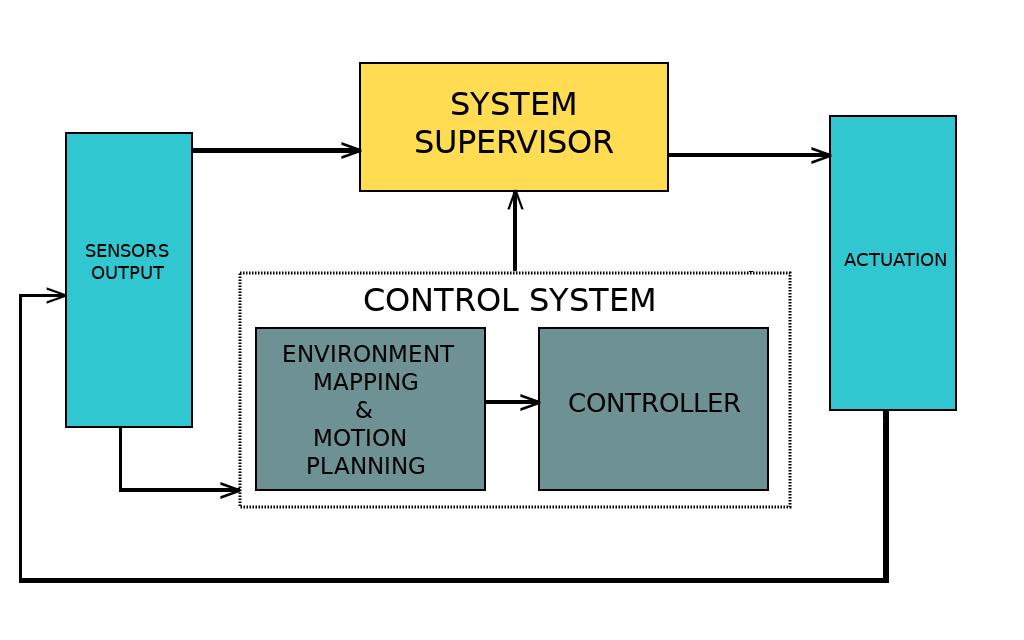
\includegraphics[width=\textwidth]{img/av-architecture.png}
	\caption{High-level abstraction of the system's software architecture}
\end{figure}

Data from sensors are inputs of the control system, here simplified as composed by two constituent systems: one in charge of collecting data directly from the sensors, process them in order to build an \textsl{occupancy grid}\footnote{A matrix mapping the environment, the cells $a_{i,j}$ are flagged with 0 if there's no object at coordinates $i,j$, 1 if occupied.} to map the surrounding area and to create a physical model of the environment in order to follow the correct route to the destination without crashing. The Controller (usually composed as a combination of a Velocity Controller\footnote{Controller in charge of adjusting the vehicle's speed} and a Steering Controller\footnote{Controller that determines the steering angle}) uses these data to adjust the values on the actuators controlling the movements of the car: throttle, brake and steer.\newline
Due to the criticity of their task, it's mandatory to have a System Supervisor, a System in charge of detecting possible hardware failures or wrong outputs\footnote{With \textsl{"wrong"} is intended not only outputs out of the domain space but also outputs that would cause the system to fail (e.g. causing a crash)} from the Control System and, if needed, activate a corrective routine.

The System Supervisor is the main failure avoidance component of such systems. Of course there may be specific checks when data are processed, but the last decision is up to this system's monitor and the underestimation of its importance can lead to dramatic consequences, such as the 2018 accident in Arizona, where a woman was killed by a self-driving car during a test run.\cite{arizuber} Further inspections showed that the car's radar and LiDAR sensors detected the victim almost 6 seconds before the impact and it took 4 seconds circa to infer that there was an obstacle on the road and that an emergency brake was needed. However, this safety-checker was disabled during tests for "smoother rides", causing the accident.\cite{govarizuber}\newline\newline
The extreme complexity of these systems raise concerns among the experts: the need to find a new point of view to study and test the safety of these systems, and the need to sensitise about safety culture.\cite{koopman}


\section{Safety And Autonomous Vehicles}

According to a SAE International tentative to classify self-driving cars' autonomy, the level of automation can be divided in 6 tiers, ranging from 0 to 5. Level 0 means no autonomy: a human driver just drives the car; level 5 means that there's no need of human intervention at all and the car is not only capable of driving safely on the road, but it must be able to avoid catastrophic failures that may seriously harm (or kill) people.
The more autonomous the car is, the higher the dependability requirements are for it to be put on public roads.
It is a well known issue that demonstrating a system's dependability is not an easy task for itself, it gets even harder with ultra-high dependability systems such as these are. In adition to the problem itself, demonstrating autonomous cars' dependability has two more problems to deal with: how to safely and effectively test the system and the presence of neural networks, for which it's very hard to understand why it returned the output $y$, given the input $x$.

Lots of studies demonstrated that it's unthinkable to just test cars on the roads. One of these, that we will refer to as the RAND Study, answers the question of how many miles of driving would it take to demonstrate autonomous vehicles' reliability using classical statistical inference, saying that if autonomous cars fatality rate was 20\% lower than humans', it would take more than 500 years with \textsl{"a fleet of 100 autonomous vehicles being test-driven 24 hours a day, 365 days a year at an average speed of 25 miles per hour"}.\cite{randstudy}\newline
The validation of ultra-high dependability requirements for safety-critical systems is a well known problem in safety literature and has not been introduced by the advent of autonomous cars. In fact, the RAND study is nothing but a specific case of the problem considered in a work published in 1993 by Littlewood \& Strigini, in which the same concepts are discussed and generalized for every ultra-high dependability system.\cite{littlewoodStrigini}\newline
The main problem with the RAND study approach is that future failures frequency can not be predicted just using the observed one. Not just for the quantitative results of the impossibility of it, but also because this approach can not work: an observed frequency failure of $0$ would lead to optimistic (and probably harmful) predictions. Luckily, this problem is surmountable, as shown in \textsl{this}\cite{zhaoStrigini} work by Zhao et al.\newline

Validating the dependability requirements of an autonomous car seems a hard task already. Things are made even harder by the fact that these cars are driven by neural networks.\newline
In these years there is a huge growing interest in the \textsl{machine learning} sector, and this has made that a lot of progress was done in the research. It's also thanks to these progresses that autonomous cars now seem like something we can achieve, since these AIs gave surprising results with their skills, and big brands such as \textsl{Uber} and \textsl{Tesla} are putting more and more efforts in AI research.
This new wave of AI research is deeply changing the way we interact with computer systems, and surprising results were achieved with neural networks.\newline
These tools have proven to outclass \textsl{"classic"} software solutions (intended as non-neural network) in a lot of tasks, ranging from \textsl{Object Detection}\cite{retinaNet} to \textsl{Gaming}\cite{alphaGo} problems, performing even better than humans.\cite{alphaGoBeatsMan}
The complexity of the environment in which the system performs and the need of quick decision-making procedures and fast responses to events that \textsl{cannot} be planned with \textsl{"classic"} software, make neural networks the perfect tool to achieve the task of a car being able to drive by itself, thanks to their ability to handle multiple situations that were not explicitly written in the software. However, this raises serious issues about the safety of the whole system for many reasons.\newline

If neural networks gave promising results on one hand, and they seem the only way to achieve goals such as autonomous cars, on the other hand it has been shown many times how weird a network's prediction can get when \textsl{minimally} perturbating the inputs\cite{stupidnn} and how high the confidence interval can be.\cite{foolnn} The lack of official regulations and certifications for this kind of software, as well as the need to truly understand neural networks, is raising concerns on how dependable these systems can be and consciousness is now growing on the topic, asking for more regulations on companies developing advanced AIs.\cite{elonmusk}\newline

\section{Controller - Checker Problem}


The interaction between the Control System and the System Supervisor is at the core of the car's movements. The Control System, or \textsl{Primary Component}, is the software performing the main computations of the system, required to drive the car. In a context like this, it's mandatory to have fault-tolerance mechanisms such as the System Supervisor, to avoid catastrophic failures. This kind of architecture is a must for these systems, due to the extremely high dependability requirements they have, in order to try to cover all the possible failures that may happen. The state space of such systems may be sketched as in figure 7.

\begin{figure}[h!]
	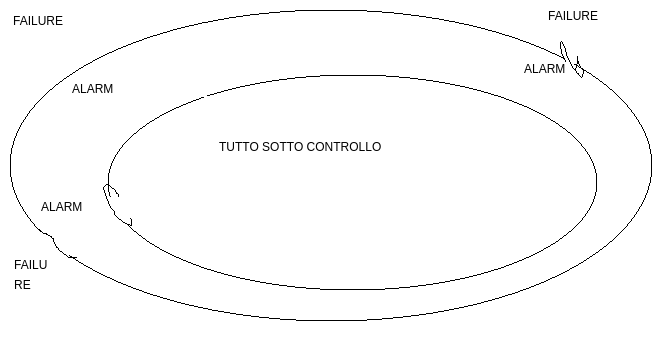
\includegraphics[width=\textwidth]{img/state-space.png}
	\caption{Sketch of the system's safe states}
\end{figure}

We consider \textsl{safe states} all the states in which the Control System produces an output that would not result in a crash.

Imagine that an autonomous car is riding when suddenly an obstacle appears. If the Primary correctly detects the obstacles it should aoutonomously apply a safety-measure to \textbf{avoid} a transition in an \textsl{alert state}. If the controller doesn't see the obstacle, \textsl{or} detects it but keeps throttling, there is a transition from a \textsl{safe-state} to an \textsl{alert-state}, in which the failure-avoidance components turn in. The System Supervisor's duty is now to launch a corrective-routine that will put the system in a fail-safe state (e.g. by applying the safety-brake and turning off the engine). An error of the Supervisor will inevitably cause the system to fail, as a result of the failure of both components, leading in a failure state (the crash happened). If we model the system's failures in this way, the level of safety of the system can be represented as the union of the failure area covered by the Controller and the one covered by the Supervisor

This problem is nothing but a generalization (related to safety) of the asymmetric fault-tolerant architecture for computer systems: the idea of having a \textsl{Primary Component} that performs the main computations, and a \textsl{Primary Checker} in charge of detecting (and correcting) possible errors of the Primary.\newline
The problem of assessing the dependability of these simpler (but still complex) systems is a well known topic in literature and was explored in different studies. In a relatively recent work published by \textsl{Popov} and \textsl{Strigini} in 2010, it is shown that the probability of a system failing on a specific input (or set of inputs), strictly depends on both the coverage of the Primary \textsl{and} the Primary Checker, as shown in the figure above.\cite{striginiPopov}

In the context of self-driving cars we want the area covered by the primary to be the largest possible. This is done by intensive training of the neural networks that will control the car. As long as the network is trained \textsl{"properly"}, the control system should be able to handle most of the dangerous situations that may happen. At one point, it is possible that the Controller learns to handle the \textsl{"alert states"} covered by the System Supervisor, reducing the overall contribution to the system's safety given by the latter.

Another possibility is that during the training, a portion of the failure area covered by the controlller becomes uncovered. This could result in a situation in which some of the previously safe states are now alarm state, representing a serious harm to the system's dependability. Since the coverage area provided by the System Supervisor can not change without changing its implementation (it doesn't "learn" automatically), a transition to one of these states would now inevitably result in a failure.

All these considerations and the lack of literature on the topic for these new systems such as autonomous cars, lead us to begin a study on the emergent behaviour resulting from the interaction of a neural network control system and a \textsl{"classic"} error checker, on what happens when the network is \textsl{taught} by a supervisor during the training and how performance metrics of these 2 components can be computed.\newline

In the next sections we present and discuss the development and implementation of an experimental methodology to study these aspects.

\begin{minipage}[c]{\textwidth}
	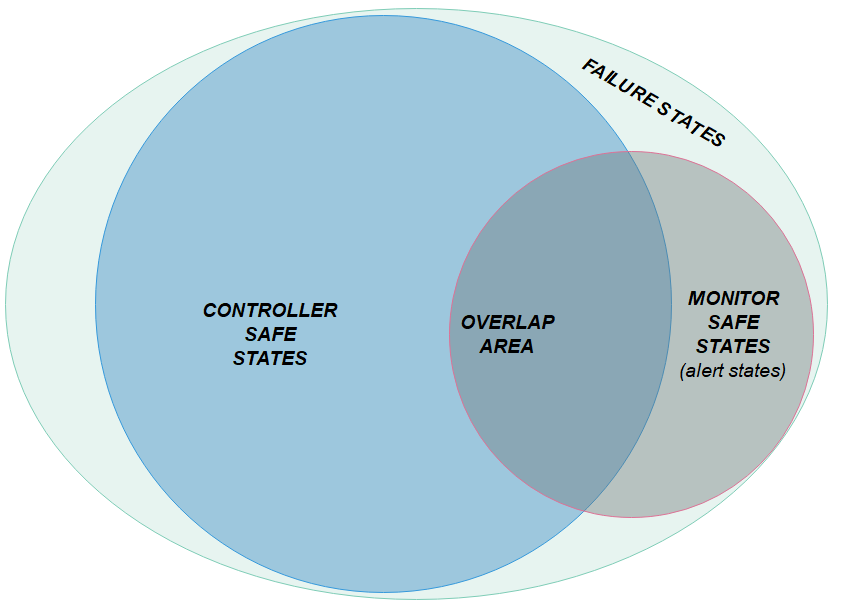
\includegraphics[width=\textwidth]{img/area-growth-good.png}
	\captionof{figure}{The states covered by the Controller are now the ones previously covered, plus some states previously covered just by the Monitor}
	\vspace{0.5cm}
	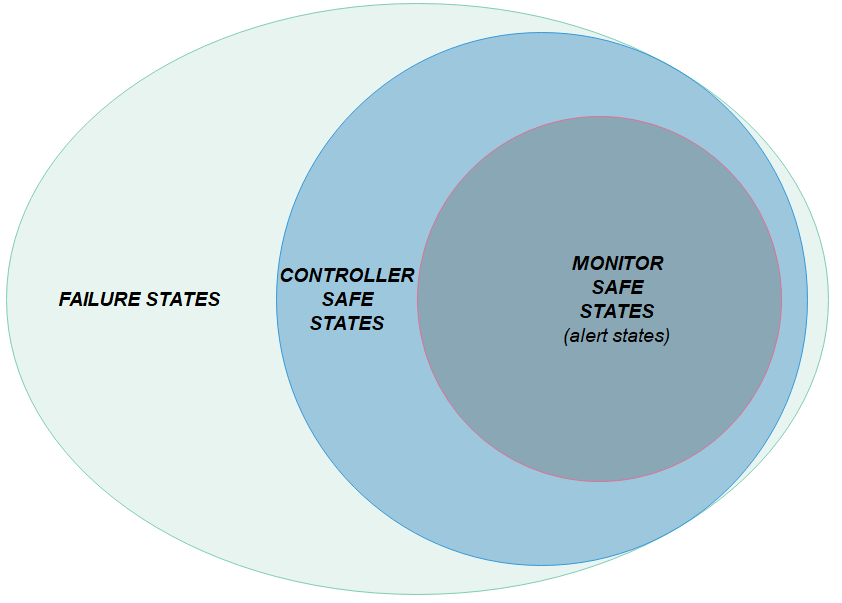
\includegraphics[width=\textwidth]{img/area-growth-bad.png}
	\captionof{figure}{The Controller now covers all the states previously covered by the Monitor, but doesn't cover anymore some of the states he covered before the training}
\end{minipage}

\chapter{System Analysis Method}

\section{Introduction and Preliminaries}

The goal of this study is to develop a first experimental methodology intended to observe emergence-related aspects coming from the interaction of a Control System and a System Supervisor, analyzing the system in a \textsl{simulated} environment.\newline
The software architecture of an AV was simplified in two main components:

\begin{itemize}
	\item A \textsl{Controller}: a Neural Network trained with \textsl{reinforcement learning} algorithms to drive the car
	\item A \textsl{Safety Monitor}, a submodule of the System Supervisor, that checks whether the car is going too fast towards an object, processing data received from a LiDAR sensor, and if that's so, apply an emergency-brake
\end{itemize}

This work focuses on exploring the topic from a different point of view and to assess its feasibility in an experimental, simulated environment. Due to the system being composed by two constituent systems: the Controller and the Monitor, we think that a point of view based on the emergent behaviour resulting from the interaction of these systems can improve the quality of the assessment.

In this chapter is presented and discussed a method to study the safety level of an autonomous car over time, observing the emergence resulting from the interactions of a neural network controller and a safety monitor in a simulated environment.

The proposed framework is designed with particular attention on studying the emergence resulting from the interaction of these two consitutent systems.

The main aspects we are interested in this first stage of exploration are:

\begin{itemize}
	\item How the effectiveness of a monitor evolves when the neural network is learning
	\item Effects of training strategies on the effectiveness of a safety monitor
\end{itemize}

One of the most appealing features of neural networks is that they can be \textsl{trained} on data sets to improve their performance. One stage of training is done by collecting data over \textsl{n} steps and updating the weights of the prediction function. The weights of the function after $i$ training stages represents the \textsl{state} of the network at \textbf{epoch i}.\newline
A neural network will likely give good results after "enough" epochs. The harder the task, the more epochs are needed. Driving a car is a quite hard task and it's inimmaginable to save the weights of each epoch. Therefore, given a neural network N, we define a \textbf{checkpoint} as a generic epoch of N. Say we trained N for 1000 epochs. If we save the weights of the prediction function every 100 epochs, we will end up with 10 checkpoints:

\begin{center}
	$checkpoint_{1}\: <\: checkpoint_{2}\: <\: \dots \:<\: checkpoint_{10}$
\end{center}

where $checkpoint_{1}$ contains the network's weights at epoch 100, $checkpoint_{2}$ at epoch 200 and so on.\newline

Let's now consider a self-driving car that is being tested on the road (either real, or simulated). Its task is to ride the car the longest possible, without crashing. During the ride, the environment surrounding the car will change as it procedes in its run. It may happen that in some of the system's state, the probability of a subsequent crash becomes very high, like a pedestrian suddenly crossing the road, if and only if the action taken by the Controller would result in the pedestrian getting hit we will address it as a failure (of the controller). The same reasoning applies if the pedestrian is actually detected, and the car hits something else while trying to prevent it:

\begin{itemize}
	\item If the Controller takes \textsl{any} action that would result in a crash, it's considered failed
	\item If a hazardous event happens, i.e. a situation in which the probability of observing a crash is higher than usual, the Controller is considered failed if and only if its actions will not avoid the imminent failure
\end{itemize}

In this sense, at this stage of the work, we don't distinguish between changes in the environment that raises the probability of a crash (e.g. a pedestrian crossing the street) and hazardous actions take by the Controller (e.g. a sudden steer towards a wall).

If the controller fails in the way just described, it's the Monitor's duty to run a safety-routine in order to prevent the imminent failure.\newline

In the case of a failure of the Controller, the Monitor not only needs to detect whether it failed or not, but it also must run a safety-routine to prevent a failure of the whole system. In this first phase of analysis, we consider the action taken by the Monitor to be always safe. This means that:

\begin{itemize}
	\item If the Monitor executes \textbf{all} the steps in the safety-routine, the system will be in a safe-state.
	\item A failure of the Safety Monitor may be one of the following:
	\begin{itemize}
		\item[1)] The obstacle is not detected
		\item[2)] The obstacle is detected but the routine fails to terminate its execution (i.e. the detection was too late)
	\end{itemize}
\end{itemize}

We consider the system failed if and only if both the Controller and the Safety-Monitor failed, as described above, leading to a crash.
With this scheme in mind, the states space for this system can be modeled in this way:

\begin{figure}[h!]
	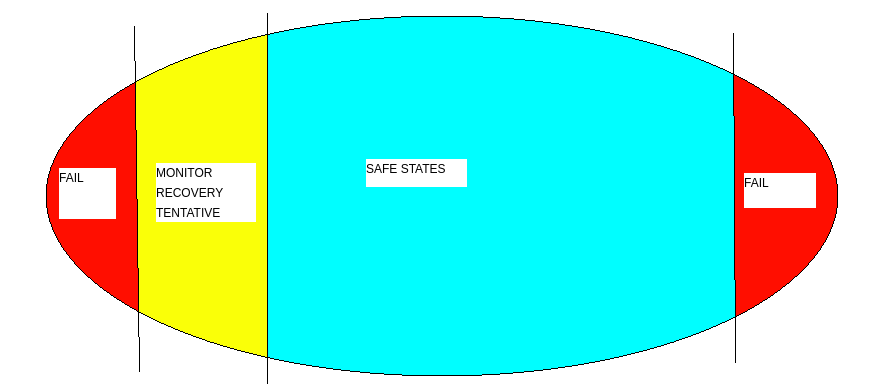
\includegraphics[width=\textwidth]{img/state-space-true.png}
	\caption{The light blue area contains the states in which the Controller is \textsl{"in control"} of the situation: the action taken by the Controller \textbf{will not} cause a Failure. The Yellow area represents the states in which the Controller made a \textsl{"wrong"} action, and without the intervention of the Safety Monitor, the System would inevitably fail. The red areas represent the fail-states.}
\end{figure}

As it's shown in this figure, we can classify the states of this system in 3 sets:

\begin{itemize}
	\item Safe States: states in which the Controller doesn' need an intervention of the Monitor
	\item Alert States: states in which the Monitor is required to intervene. A correct detection (and prevention) of the potential accident would result in a transition to the safe states space again
	\item Failure States: states in which an accident happened. It is important to notice that \textbf{not} all the situations can be detected by the Monitor. There are accidents that can not be prevented at all, in which no Monitor could save the system. These states are represented by the red area on the right
\end{itemize}


At the system level, we are interested in observing the probability of having a failure (crash) and how to minimize it. At the same time we want to observe how the effectiveness of the Safety Monitor changes when the Controller is trained over time.

In order to achieve this, $c$ checkpoints are saved for later testing and comparison. This is useful not only for checking that the network is improving during the training, but also to have a better understanding on how useful is the Monitor when the Controller becomes more and more expert. This is mandatory for the experimental activity as different checkpoints of the same network are tested under the same condition, to observe how the behaviour of the Controller changes in the first stages of the training.

The need for multiple checkpoints is mandatory not only to test that the network is improving, but also to observe how the monitor's effectiveness change over time. Moreover, if many checkpoints of the same network are tested under the same scenarios, it is possible to extract interesting measures, as we'll see in the next section.

Before the analysis can start, $n_{h}$ scenarios must be defined. A \textsl{Scenario} is a set of initial conditions (e.g. the spawn point of the car, seeds used in random number generators$\dots$) in which the car is intended to be tested. The pedix $h$ represents the difficulty level for the specific case. The purpose of this is that we are interested in testing the car under the same initial condition but for one factor, in order to have a better understanding on what makes the system fail more often. The $h$ variations should be developed with growing difficulty and at the same time they must be realistic. Given a Scenario $S$, examples of variations may be: to increase the number of cars in the scenario, or to simulate adversal weather conditions. A combination of these 2 variations should result in a \textsl{harder} variation of the scenario\footnote{It is important to point that what we think to be "harder", may in reality be easier to handle for the car.}. It's important to keep in mind that these scenarios, once defined, should not be changed as they will be used for testing all the checkpoints. A change in the settings of a scenario (except for variations) should be considered as a new one.

We hope that the results collected here will help in the process of understanding what makes a situation \textsl{"harder"} than others for such systems.

\section{Experimental Method}

The approach used for this exploratory work is divided in 3 phases:

\begin{itemize}
	\item Phase 1: Given $c$ checkpoints of a neural network and $n_{h}$ scenarios, the Controller is tested in all the scenarios and its runs are recorded
	\item Phase 2: The Monitor is tested by \textsl{repeating} the runs recorded in phase 1, attaching the Safety Monitor to the system
	\item Phase 3: The network is retrained from the last checkpoint recorded, using different strategies to improve its performances. The new networks obtained and the (same) Safety Monitor are then retested in all the $n_{h}$ scenarios
\end{itemize}


In the first phase we are interested in assessing the goodness of the neural network and of the Monitor. This is done in 2 different steps. 

In the first step, the $c$ checkpoints of the Controller are tested in all the scenarios. In this step we are mostly interested in observing how the \textsl{Reliability} of the Controller changes with respect to these checkpoints.

One of the main problems when testing a neural network is that of \textsl{repeatability}. It is very unlikely that the \textbf{same} neural network, under the \textbf{same} initial conditions, will behave in the same manner in multiple runs. Due to this property of networks, it may happen that the failure mode observed in one of the runs of the scenario $s_{i}$ will never happen again, or the time needed to make it happen again may be very long.
How the scenarios and their variations are created is fundamental to observe specific failures, however it's impossible to think to \textsl{all} the possible failure situations that may happen, for this reason we think that the scenario-variation approach may help in solving this issue, creating harder operational situations in which the factors that lead to a crash may be studied.

The repeatibility issue was solved by creating a \textsl{black box} for each run of the scenarios developed for testing. This approach is used to keep a trace of the Controller's actions, so that the specific run may be studied more fully to understand what made tha Controller fail. These data can be then used to better study what hazardous situations are covered by the Controller at a specific checkpoint $j$, and if these situations are still covered when the network is tested at the checkpoint $j+x$.\newline


\subsection{Controller Testing}

The Controller is tested in isolation in each scenario, for each difficulty level, until a crash occurs. The situation in which no failure is recorded is still a possibility (even if the difficulty level somehow mitigates this issue). A reasonable alting criteria is out of the scope of this work and is still a problem in the academic community, however, as noted in the previous section, this problem may be solved.\cite{zhaoStrigini}

The reasoning behind the choice of isolating the in order to test it Controller, comes from some of the problems issued during the method development phase.
The main problems are the \textsl{repeatibility} and \textsl{non-intrusiveness}. As pointed before, the \textsl{repeatibility} issue for the neural network is solved by creating a \textsl{black box} containing informations about the car's state in each frame. At the same time we can not think about testing the whole system at once (Controller \textsl{and} Monitor) because a safety-brake executed by the monitor will most likely change the environmental conditions for the rest of the simulation and we would not be able to compute measures about the goodness of the Controller itself. Testing the Controller in isolation helps to solve these issues and it's preparatory to the second phase.

Recording the actions taken by the Controller for \textsl{each} frame (as well as other measures such as the vehicle's speed in that frame) make it possible to have a great control over the data, as a single run may be repeated many times to gather additional data if needed.

When the controller has been tested for each difficulty, in all the scenarios at least the followings must be computed:

\begin{itemize}
	\item $MDBF_{i,j} = \frac{\#\: of\: faults}{meters\: travelled}$
	\begin{itemize}
		\item[-] Mean Distance Between Failure for the $i^{th}$ checkpoint, at the $j^{th}$ level of difficulty
	\end{itemize}
	\item $MTBF_{i,j}\: =\: \frac{\#\: of\: faults}{operational\: time}$
		\begin{itemize}
		\item[-] Mean Time Between Failure for the $i^{th}$ checkpoint, at the $j^{th}$ level of difficulty
	\end{itemize}
	\item $FR_{i,j}\: =\: \frac{1}{MTBF_{i,j}}$
	\begin{itemize}
		\item Failure Rate of the $i^{th}$ checkpoint at the $j^{th}$ level of difficulty
	\end{itemize}
	\item $R_{i,j}(t)\: =\: e^{-FR_{i,j}\cdot t}$
	\begin{itemize}
		\item Reliability Function of the $i^{th}$ checkpoint at the $j^{th}$ level of difficulty, i.e. the probability that the Controller $C_{i}$ is not failed at time $t$ when operating at difficult $j$
	\end{itemize}
	
\end{itemize}

When measuring the reliability function $R(t)$ of a system, one of the main measure of interest is its Mean Time To Failure, because it is easy to compute in simulated environments, and it's used to compute the rate $\lambda$ of the exponential function.
In the Automotive Sector however, data are usually computed with respect to the travelled distance, i.e. Mean Distance to Failure, rate of crashes per kilometers, and so on.
With our approach, if the simulated environment and the hardware running the simulations are powerful enough to run the simulations at a fixed time-step, it's very easy to switch the point of view on the data.

As long as the neural network is trained properly, we expect the following disequation to hold: $R_{i}(t)\: \leq \: R_{j}(t)$, where $i$ and $j$ are 2 checkpoints, with $i\: <\: j$. This can be easily verified using the approach defined above to collect the data.

\begin{figure}[h!]
	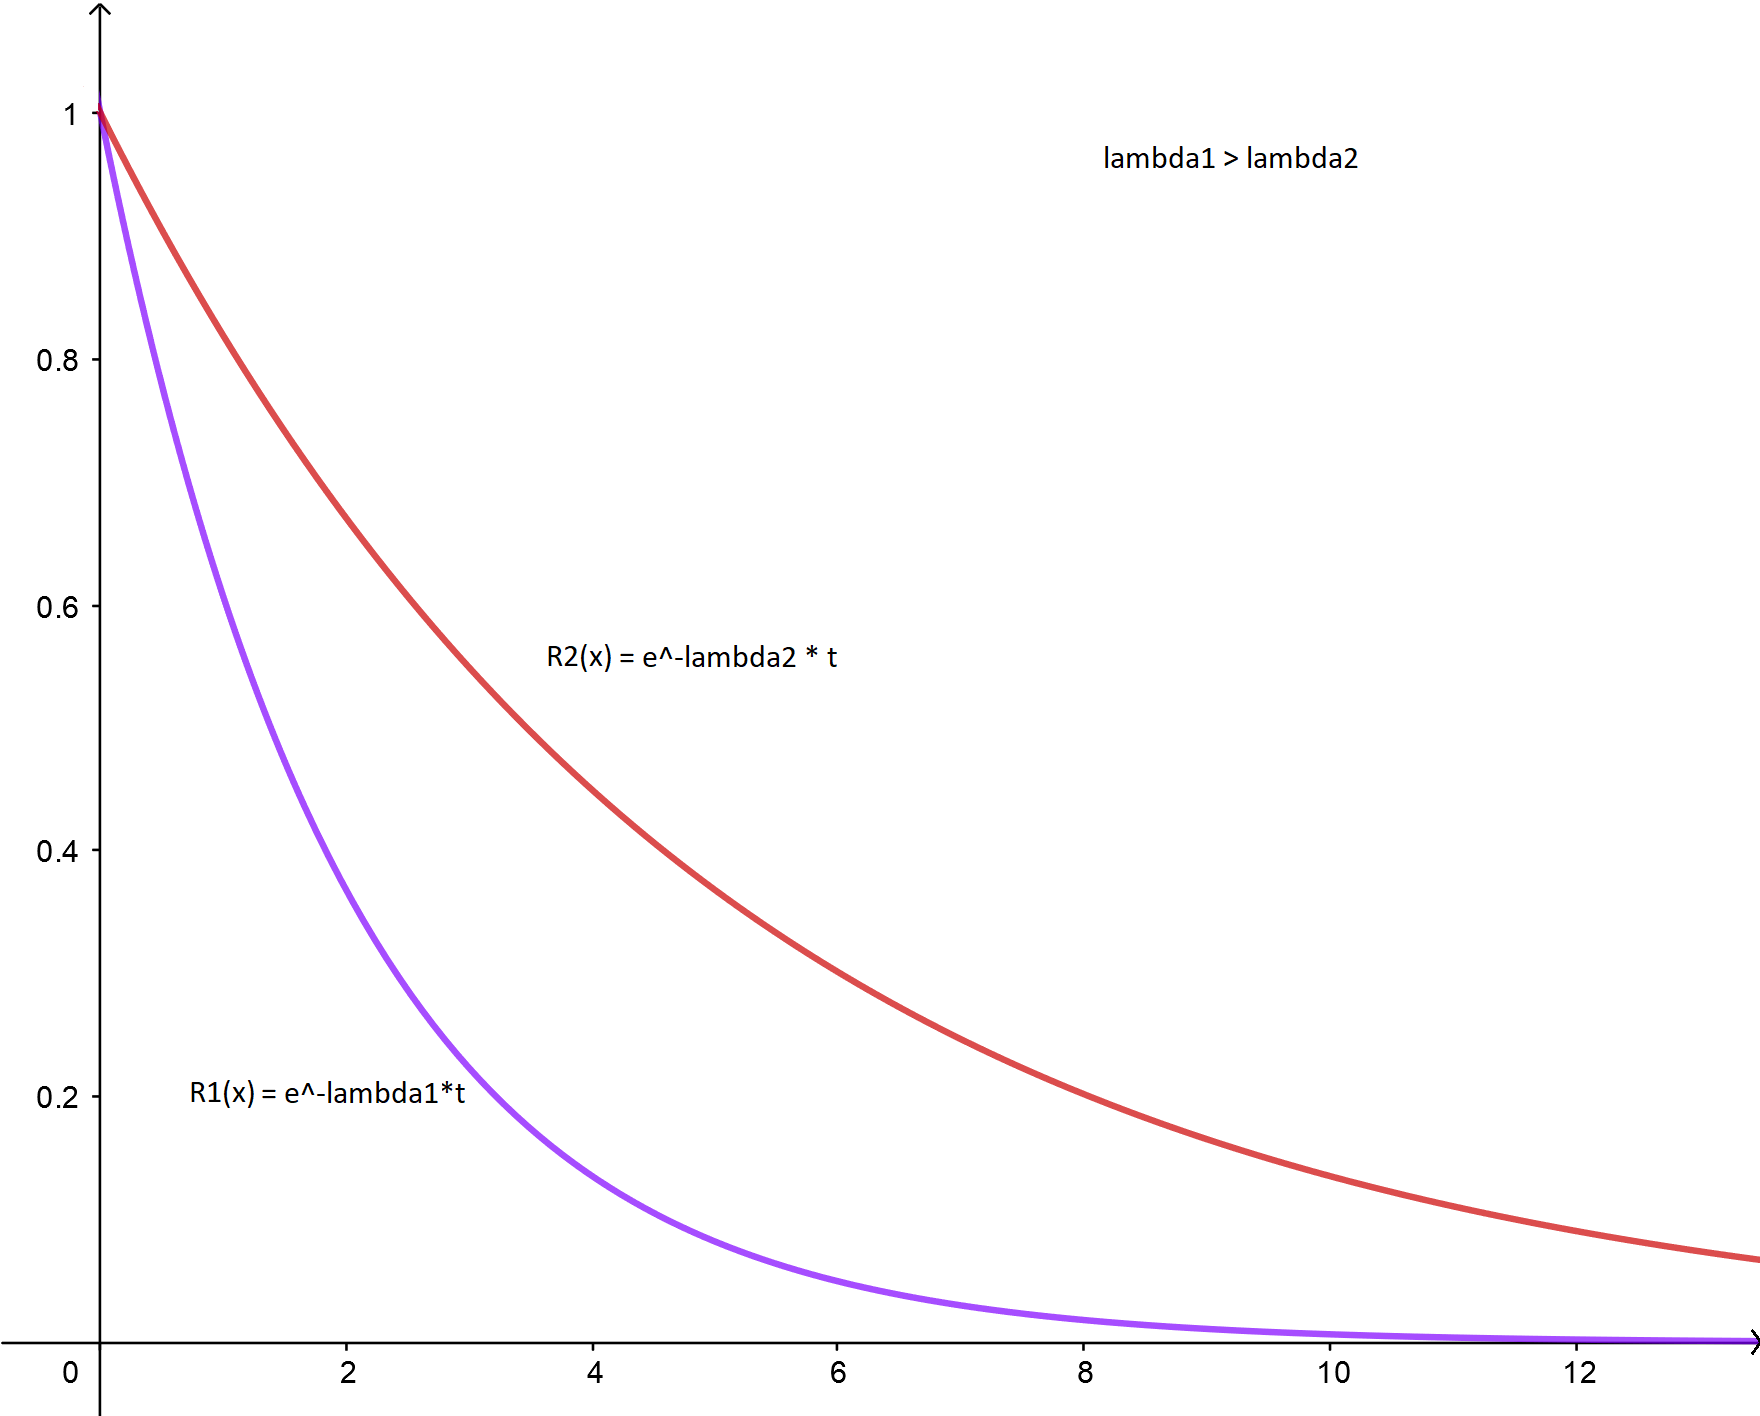
\includegraphics[width=\textwidth]{img/reliability-curve.png}
	\caption{The Reliability function measures the probability that at time $t$ the system is still operating. We expect that more expert drivers (i.e. more trained networks) are capable of longer runs than little trained networks}
\end{figure}

\newpage

If the Simulator used for testing permits it, other data should be recorded too, in order to enhance the comprehension of the Controller's behaviour, such as:

\begin{itemize}
	\item The car's instantaneous speed and acceleration vector at each frame
	\item With \textsl{what} the car crashed (e.g. a vehicle, a pedestrian, a generic obstacle$\dots$)
	\item Environmental conditions at time $t-x$, if a crash occurred at time $t$
\end{itemize}

These data are fundamental to distinguish between \textsl{"safe"} and \textsl{"catastrophic"} failures. For example, if a fence is hit at a speed, let's say, less than 10km/h, it may be flagged as a less serious crash than hitting a pedestrian at the same speed.

As the Controller learns, we expect the \textsl{Reliability Function} and the \textsl{MTBF/MDBF} to increase, since a trained driver should in principle cause less crashes than a non-expert one, therefore increasing the value of the MTBF and possibly the y values of $R(t)$.

If the \textsl{black box} makes use of enhanced data (such as the ones listed above), it is also possible to observe changes in the car's behaviour with respect to the scenario and the difficulty level. For example: if we define a difficulty $k$ by doubling the number of cars in the scenarios, it may happen that it is observed an increasement on the amount of collisions against other obstacles. If that's so, the simulations should be studied more deeply to enforce the training strategy in a certain direction, as this may mean that the Controller is going to crash on walls while trying to avoid other vehicles.


\subsection{Monitor Testing}

Once the Controller's runs are recorded as described previously, the Monitor testing can start.

The goal of this phase is not only to see how good the Safety Monitor is in preventing crashes, we are also interested in observing evidences about which situations are \textsl{"hard"} for the Monitor, and which for the Controller. 

As the network becomes more expert, it may happen that its behaviour evolves in a way such that the Monitor is no more able to detect imminent failures, because the Controller is now good enough to cover all the failures previously covered by the Monitor, and the hazards caused by its novel behaviour are such that the Monitor is not able to detect them.

However, the opposite is also a concrete possibility. For example, in the first epochs the Controller may drive in a "crazy" manner, e.g. with a lot of sudden, high-angle steerings and riding at high speed. The Monitor will obviously have more problems in predicting what the next state will be due to the unpredictability of the Controller's behaviour. The more the network learns, the more it will (hopefully) ride smoothly, making it easier for the Monitor to detect possible, imminent crashes.

The main problem that should be addressed here is that the Monitor effectiveness may decrease, while the network is learning, resulting in a useless component that may even be detrimental to the system's \textsl{performability}: the Controller may become good enough to be able to cover all the hazardous events covered by the Monitor at an earlier checkpoint. This may not change the whole safety of the system, if we consider the actions taken by the Monitor as inconditionally safe, but it would result in lesser smooth rides, due to the safety-brakes applied by the Safety Monitor.

The Monitor is tested as follows: the black boxes create during the Controller testing phase are used to \textsl{repeat} the runs. The initial conditions must be \textsl{identical} as well and should be saved as part of the black box in the previous stage. The runs of the Controller previously recorded are now repeated, attaching the Monitor to the System and recording the alarm raised during the run and if it was able to prevent the crash that originally occurred.

In this stage of the analysis, the major concern was that of \textsl{non-intrusiveness}. For the reasons pointed above, we can not think about rerunning the simulations just by attaching the Safety Monitor and watch how it goes. The Safety Monitor, by definition, \textsl{overwrites} the Controller's action if an alert is raised, changing the next part of the run. This is theoretically not a problem, if one can distinguish between false and true positives. However, we can not know in advance what a false positive will be without creating a software capable of sensing an mapping the environment. But this is a Safety Monitor itself and, as every tool of this kind, it will have false positives even if extremely low, therefore this approach can not solve the problem.

The idea is to record the alerts generated during the run, without enabling the safety-procedure (e.g. the brake). Since we are going to repeat exactly the runs recorded in phase 1, it's possible to know the instant of time $t$ in which the transition to the \textsl{alert state} before the crash occurred. With this information, all the alerts raised before $t$ are indeed false positives, or false alarms, since we know $t$. Enabling the Monitor to activate the safety-procedure after this instant of time, makes possible to approximate its coverage. 

Recall that what we call a \textsl{"failure"} of the Controller is a transition from a \textsl{safe state}: a state in which the Controller can handle what's happening in the environment without crashing, to an \textsl{alert state}: a condition in which without a Safety Monitor, the System would inevitably go to a failure state.
For this component, we want to measure its ability to distinguish between safe states and alert states. To do so, we defined positives and negatives predictions in this way:\newpage

\begin{itemize}
	\item[TP:] True Positive
	\begin{itemize}
		\item[-] The system went in an alert state due to a Controller's failure, correctly detected and prevented by the monitor
	\end{itemize}
	\item[TN:] True Negative
	\begin{itemize}
		\item[-] The system is in a safe state and the Monitor doesn't raise any alarm
	\end{itemize}
	\item[FP:] False Positive
	\begin{itemize}
		\item[-] The system is in a safe state, but the Monitor raises an alarm
	\end{itemize}
	\item[FN:] False Negative
	\begin{itemize}
		\item[-] The system is in an alert state and the Monitor doesn't detect the hazard
	\end{itemize}
\end{itemize}


\begin{figure}[h!]
	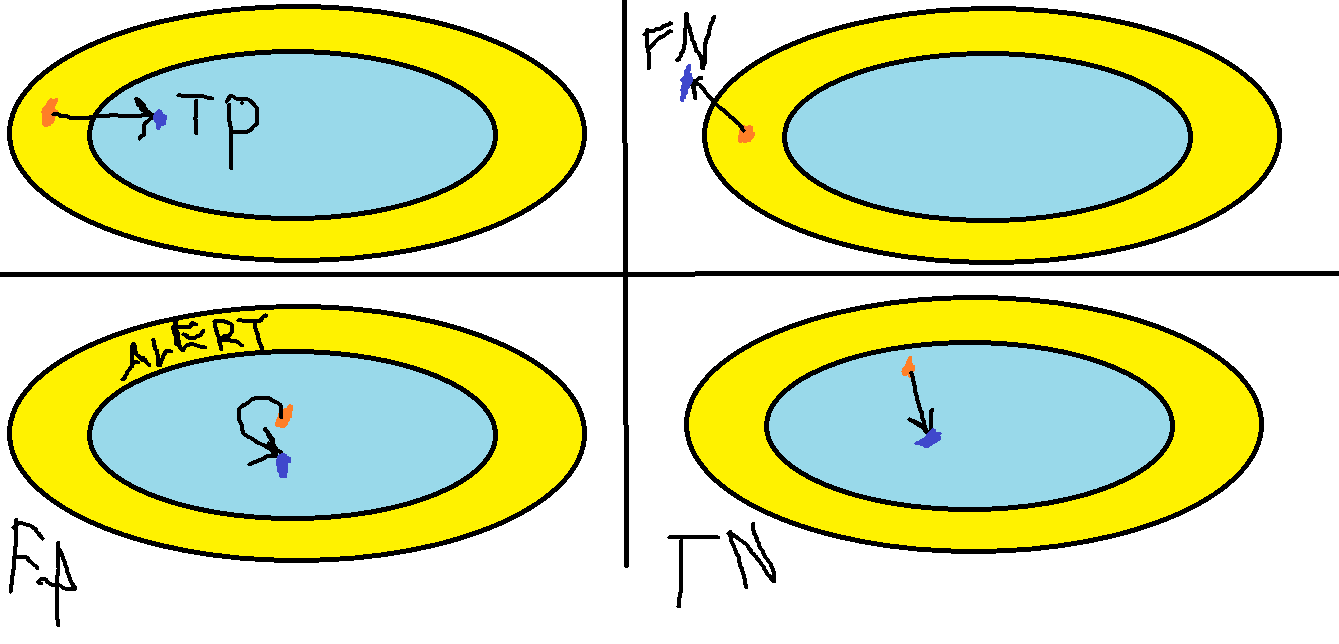
\includegraphics[width=\textwidth]{img/positive-negative.png}
	\caption{Graphical Representation of what true and false predictions means in the system's state space. Recall that the light blue area is the set of \textbf{safe} states, and the yellow area represents the \textbf{alert state}, in which the Monitor intervention is \textbf{mandatory} to a void a system failure}
\end{figure}


These measures are commonly used to see how good a model is in classification problems. However, for real time critical system it's not easy, if not impossible, to measure all of them. In particular, it's not always possible to understand when the Controller avoided a crash and the monitor \textsl{did not} raise an alarm. This issue makes very hard to measure the amount of true negatives because in most of the cases, this kind of situations may be seen only when a human operator analyse the specific run.

In particular, an input for the Safety Monitor is composed by multiple, timed inputs, that can be seen as the evolution of the environment while the system is performing its operations. For this reason, it is hard to understand whether the next state will be an alert or a safe state because we don't know \textsl{when} the series of inputs that will eventually result in a crash will begin.

This puts some limits on the metrics and the ratios that can be computed for the Monitor as they require the amount of true negatives. However, fortunately, a true negative does not change the behaviour of the system because there is no safety-brake, therefore after some analysis it was decided to ignore the true negative rate. At the same time, we want to observe at least the amount of false positives and convert it to a rate, for the purpose of comparison.\newline

Since we do not know the \textsl{real} amount of \textsl{True Negatives}, for the reason just described, some of the measures usually considered when assessing the prediction performances of a model could not be approximated. To give a rate measure for false positives, it was decided to compute the amount of false positives over the distance travelled in a run.

\begin{itemize}
	\item True Positive Rate:
	\vspace{-0.5cm}
	\begin{center}
		\begin{equation}
		TPR\: =\: \frac{TP}{TP\: +\: FN}
		\end{equation}
	\end{center}
	\item False Negative Rate:
	\vspace{-0.5cm}
	\begin{center}
		\begin{equation}
		FNR\: =\: \frac{FN}{FN\: +\: TP}\: =\: 1\: -\: TPR
		\end{equation}
	\end{center}
	\item False Positives per Meter:
	\vspace{-0.5cm}
	\begin{center}
		\begin{equation}
		FPM\: =\: \frac{FP}{meters\: travelled}
		\end{equation}
	\end{center}
\end{itemize}

These rates gives a good approximation of the Monitor's behaviour and these measures can be used for the purpose of comparison.

When testing the Monitor, it is advisable to \textsl{"stress"} it under detrimental conditions, in order to collect more possible evidences and linkage among the data. Note that this aspect is independent from the \textsl{difficulty level} defined above, as it is something related to the environment itself that may give evidences about the \textsl{situations} in which the Monitor performs well, and those in which it doesn't (e.g. think about a LiDAR sensor in a very rainy environment: the observations will likely to be fuzzy/noisy) and it is more related to \textsl{fault injection} at a higher level.

The ways in which the parameters of a Safety Monitor can be tuned really depend on its implementation, and it's up to the developing team the decision on what and how many faults inject in the software. A very simple example can be that of reducing the amount of data read by the sensors (which will result in low-quality data and a poor mapping of the environment), or introduce some noise in the observations.

Doing this step when testing the Monitor allows also to understand how to tune the internal parameters of the software in order to have its \textsl{"best"} version, that will be used in the Controller retraining phase.

\subsection{Controller Retraining}

At this point we have collected data about the behaviours of the Monitor and the Controller. In this phase we are going to study how much this values vary with respect to the learning strategy adopted, when the neural network is retrained from the last checkpoint.

As said at the beginning of this chapter, we are considering a Controller composed by a neural network, trained with reinforcement learning techniques. These kind of algorithms make use of a \textsl{reward function} to tell to the network if it's behaving \textsl{"good"} (positive value) or \textsl{"bad"} (negative value) and it is calculated at each prediction step (i.e. at each action taken by the Controller).\newline

The training function needs the following parameters, that are recorded at each algorithm iteration:

\begin{itemize}
	\item[a)] Action taken by the Network
	\item[b)] State of the network in which the action was taken
	\item[c)] Reward given for the action taken in a certain state
\end{itemize}

In this phase we want to discover how training strategies for the neural network may affect the overall behaviour of the system, with particular attention on the effectiveness of the Safety Monitor.

To start an exploration in this topic, we defined 4 strategies and the outcomes we expect after the training is completed. These outcomes are \textsl{"forecasted"} in the sense that we don't know how the network will react to a change in the training strategy, nor if the observe behaviour will be the supposed one.

The strategies developed in this method are mostly based on the reward function and on the actions taken by the network:

\begin{itemize}
	\item[S1)] The reward function is now more punitive when the car hits something, while braking is slightly more rewarded, provided that the Car won't stop moving
	\item[S2)] The Safety Monitor is attached to the system and, if an alert is raised, the action of the network is replaced by the Monitor's action (the safety-brake)
	\item[S3)] The network's action is replaced by the monitor's if it raises an alert. The network is given a positive reward for behaving like the Monitor
	\item[S4)] The training step is stopped and the network is given a \textsl{negative} reward if an alert is raised
\end{itemize}

For the first strategy we expect at least the Controller's mean time/distance between failures to be lower. With this method one is also able to see if the new Controller can avoid the crashes of previous checkpoints. Another aspect we are interested in is how the Monitor's effectiveness changes in terms of positive/negative ratios.

In the second strategy we are essentially cheating. The network is \textsl{"taught"} by the Monitor to brake whenever an alarm is raised. A possible outcome is that the alert states previously covered by the Monitor become safe states. However the Monitor's false positives will inevitably have an impact on the system's availability caused by erroneous safety-brakes.

The third strategy is pretty much the same as the second. We expect that giving a positive reward when behaving like the Monitor may increase the learning speed.

The last strategy may give the most interesting results. Giving a negative reward and alting the training step when the Safety Monitor raises an alarm, regardless if it's a true or false positive, should force the network to completely \textsl{avoid} the situations in which the Monitor intervenes. Essentially we expect that the effectiveness of the safety component will be drastically reduced.\newline

After the four Controllers are trained enough, the new systems are tested as in phase one. The same measures listed before are approximated for the Controllers and the Monitor and the results are compared with the original checkpoints.


=======================================================================

FORSE

=======================================================================

As an additional step, we are going to treat the new Controllers as a Monitor for the runs recorded with the last checkpoint, to try to observe how the states space has changed.


\chapter{Method Implementation And Results}

In this chapter the tools used, the infrastructure and method implementation and the results collected during the analysis are reviewed.

A Neural Network was trained to drive in an urban environment. Checkpoints of the network's state during the training were recorded for comparison. These stages of the network were then tested with and without a simple safety-monitor in order to provide a new point of view to study AV's behaviours.

\section{Tools and software}

\subsection{Carla Simulator}

In order to have a realistic environment, with accurate physics simulation and data sensors, the open-source simulator CARLA\cite{carla}, developed by researchers at the University of Barcellona, was used. This simulator was developed with the purpose of offering an environment where AI agents can be trained to drive, with high control of the simulation parameters and the simulation of realistic sensor, which can be tuned to increase or decrease data quality, or to inject faults.\newline
CARLA is developed with a client-server architecture in mind. The \textsl{server} is basically a game, developed with \textsl{Unreal Engine 4} in C++. C++ performances are with no doubts essential to the functionality of the server: not only the environment must be simulated (inlcuding movements of pedestrians/vehicles, weather simulation\dots), but also all the data needed from the sensors attached to the system.\newline


======================================================================================

IMMAGINE CARLA

======================================================================================

CARLA is currently at version 0.9.7 and huge improvements are done at every release, gaining more attention from the experts for its realisticity. Unfortunately, when this study started, CARLA 0.9 was recently released and the tools needed for our work couldn't be found online. Thanks to the quantity of work done for the last \textit{stable} version of CARLA, 0.8.4 was used at first.\newline
Versions prior to 0.9 have some limitations on the control one has of the simulations parameters and on the data collectable from it. This doesn't impede our study, but of course limited in some way the informations on the environment and system. Some of these problems are still present in later versions of the simulator, but most of them were solved in the transition from 0.8 to 0.9.\newline\newline
One of the main problem found was with the coordinate systems. Before version 0.9, developers were using UE4's default coordinates system which is left-handed, while the standard is considered to be right-handed. This looks like not a big deal since things could be easily solved by applying a transformation matrix. However, due to performance issues (a Python client should do the real-time processng of \textsl{loads} of data at each timestep, resulting in considerable slowdowns as a result of all the processes running at the same time), it was decided to stick with the developers' decision and convert the data during analysis phase.

All the sensors available in CARLA 0.8 were used during the experiments. These can be easily accessed via the Python APIs provided:

\begin{itemize}
	\item Cameras
	\begin{itemize}
		\item The \textsl{"scene final"} camera provides a view of the scene (just like a regular camera)
		\item The \textsl{"depth map"} camera assigns RGB values to objects to perceive \textsl{depth} of the environment
		\item A \textsl{"semantic segmentation"} is used to classify different objects in the view by displaying them in different colors, according to the object's class
	\end{itemize}
	\item Ray-cast based Lidar
\end{itemize}

The three cameras were used during the training phase of the network. Three \textsl{"scene final"} cameras are attached to the car to actually \textsl{see} the environment (one on the front and 1 per side). These cameras, combined with the \textsl{"depth map"} camera allows not only the car to see, but also to perceive distances from objects in the scenario.
The \textsl{"semantic segmentation"} provides image classification features by querying the server for ground-truth values. This is with no doubt a semplification of a real system, where the most powerful image-classification softwares are essentially neural networks. A misclassification could lead to catastrophic failures but we are not interested in their accuracy: the system's safety monitor, combining data from all the available sensors, will not "correct" the misclassification but it must react fast and safely to the consequences of it.




\begin{itemize}
	\item CARLA
	\item Nervana Systems - coach (Intel)
	\item Reti neurali su git
	\item Monitor
\end{itemize}


\section{Method Implementation}

Dedicare una sezione alle decisioni prese?

\section{Results}

\begin{itemize}
	
	\item Interazione rete-monitor
	\item Safety Monitor Implementation - obstacle detection
	\item Come vengono raccolti i dati
	\item Come vengono preprocessati
	
\end{itemize}


\chapter{Conclusions}

In this work we explored the topic of how to perform a monitoring activity on self-driving cars, controlled by a Control System (Controller) and a System Supervisor (Safety-Monitor).

This study is meant to be a first step on the analysis of \textsl{how a monitoring activity should be performed for such systems}, as they require particular care due to their complexity, and the critical issues of the environment in which they operate. Autonomous Vehicles themselves are not a new kind of systems, since they are commonly employed in military actions. However, the fact that self-driving cars will work at close contact with people and that the urban environment requires extra care in handling the moltitude of events (hazardous or not) that may happen.
Moreover, we questioned if there are relationships between the effectiveness of the Safety-Monitor component and the Controller component, when the latter gets trained for long periods, using different strategies.

In the first sections, we reviewed the main concepts of these activities, such as

\begin{itemize}
	\item The definition of \textsl{dependability} and \textsl{safety}, which are central to Safety-Critical Systems, are seen in the light of self-driving cars
	\item The problems that prevent us to deploy self-driving cars in urban environments at this level of knowledge
	\item How a wrong/poor/optimistic \textsl{dependability assessment} of these systems may have tragic consequences when these systems are deployed
	\item The problems of studying the observed emergent behaviour resulting from the interaction of two main Constituent Systems
	\item If, and in what way, the Safety-Monitor effectiveness is influenced by the performances of the Controller, in terms of:
	\begin{itemize}
		\item[-] Length of the training period
		\item[-] Strategies adopted during the training
	\end{itemize}
\end{itemize}

The development of this first methodology has taken into account the tools available for this kind of activities. Since most technologies in this field are private and proprietary, we had to look for open-source equivalents, demonstrating that it's not easy to perform these analyses in non-professional environments.

CARLA is with no doubt the best self-driving car simulator available, but it's not perfect. The LiDAR sensor bug\cite{lidarbug} would have prevented us to do this study and if it wasn't for the project developed by Zhuang\cite{carlapro}, it would have been \textsl{unfeasable} because our only alternative would have been to use \textsl{ground-truth} data, which would have been pointless for this work.

If on one hand, \textsl{Coach framework} is developed by \textsl{Intel AI Labs}, it suffers from the common issues often found in open-source project, the most evident being one of the two agents provided for CARLA, which stopped moving after few stages of training in \textsl{phase 1} (therefore unrelated to the use of Safety-Monitor).
This bug makes us wonder about the presence of other issues in the design of the training algorithm which may had an influence on the behaviours observed for $C5_{S2\dots 4}$.

Another issue that mines the usability of this framework is that the RAM is not correctly freed, eventually filling it and causing a crash of the running processes. This required us to monitor the training execution and restart it at every crash.\newline

The monitoring activity was developed keeping in mind the main properties of:

\begin{itemize}
	\item Repeatibility
	\begin{itemize}
		\item[-] By recording the Controller's execution in files, saving the action taken by the Controller in each frame and the seeds used in RNGs\footnote{Random Number Generators}, the Destination Goals and the environmental parameter of each scenario
	\end{itemize}
	\item Non-Intrusiveness
	\begin{itemize}
		\item[-] Code instrumentation, as said, may produce non-real time data or wrong measurements, due to the client-server architecture used. CARLA solves this problem by allowing users to run simulations at a \textsl{fixed time step}. However the hardware must be powerful enough to achieve the time step required
	\end{itemize}
	\item Representativeness
	\begin{itemize}
		\item[-] Representativeness of \textsl{test-cases} is one of the central problems when monitoring self-driving cars, because hazardous events may be so complex and so many that is impossible to consider them all. The definition of scenarios and difficulty level helps in this sense, providing many different sitations starting from the same scenario
		\item[-] Representativeness of the \textsl{measures} computed for the Safety-Monitor raised issues on the nature of the dataset we are working with. The choice of the measures to be used on the Confusion Matrix was explained and motivated, as well as the exclusion of the others
	\end{itemize}
	\item Feasibility
	\begin{itemize}
		\item[-] The research on the best tools to be used for this activity was not easy, due to the multitude of solutions proposed that in reality have lots of practical limitations. However, the tools used in this work allowed us to perform this activity. At the same time we can not ignore the issues found in these projects
	\end{itemize}

\end{itemize}

If the \textsl{feasibility} property is undermined by the presence of issues in the tools used, the methodology developed still proved to be an effective way of assessing the reliability of Autonomous Vehicles allowing us to approximate all the common measures of interest for these systems, without sticking to common metrics used in the evaluation of neural networks, e.g. the \textsl{Loss Function}, which indeed are powerful and mandatory measures to compute to check that the neural network is actually learning, but doesn't give any evidence at all on the goodness of the System in its entirety.

This methodology proved to be an effective mean to study the behaviour of the whole System, focusing on well-known measures used to assess a system's dependability and the Safety-Monitor's performances. The definition of \textsl{Scenarios} and \textsl{difficulties} is very useful in the understanding of what environmental parameters cause a degradation on System's performances and in the generation and analysis of \textsl{"uncommon"} situations that not always can be taken into account when designing \textsl{ad-hoc safety-cases}
\newline

The main conjecture that made us start this work, was if "static" (in the sense that they don't learn from new data) error-checkers' performances were depending on the performances of neural networks and if ad hoc training strategies have an influence as well. From the data collected it looks like the Monitor's effectiveness is likely to change with expert agents, motivating us to continue to study in deep this conjecture.

The failure of those strategies that used the Safety-Monitor to guide the training ($S2,\: S3,\: S4$) did not give us evidences on this fact, and this problem was already discussed in the previous chapter. This failure may be caused by two factors:

\begin{itemize}
	\item[1)] Misspecified reward function
	\item[2)] The training period was not long enough
\end{itemize}

The fact that the agents trained were not getting unintentionally high reward for standing still, makes us think that the neural network needed more time to learn what the Safety-Monitor is trying to teach. A higher \textsl{simulation time step} could have helped us, making \textsl{simulation time} running faster than \textsl{real time}. However, this required ultra-high performance hardware, therefore we could not train the models for more time, nor retrain the networks adjusting the reward parameters.

At the same time, the Safety-Monitor proved to be \textsl{less} effective when operating in combination with the Checkpoint which had the \textsl{best} performances and, most of all, it was the one obtained from Checkpoint $C4$ by changing the training strategy, while when operating with the Checkpoints trained with strategy $S0$ $(C1,\: C2,\: C3,\: C4,\: C5_{S0})$ it had the same TPR ($0.75$), with the exception of $C2$. If on one hand, $C2$ was definetely a special case, for the reasons listed in the previous chapter, at the same time we can not exclude the same hypothesis for $C5_{S1}$. In future works, we want to continue the training of $C5_{S1}$ to confirm this fact.\newline

This work demonstrated the power of the use of a simulated environment for the assessment self-driving cars, taking into account and solving many of the problems found when approximating the measures of interest for these systems, and common problems found in a monitoring activity.

In future works, our interest will be:

\begin{itemize}
	\item Developing stochastical models based on data collected with this monitoring methodology, to guide us in the tunning of the reward function parameters
	\item Continuing the training of $C5_{S0\dots 4}$ to:
	\begin{itemize}
		\item[a)] Collect more evidences about the effectiveness of the Safety-Monitor
		\item[b)] Have a better understanding of the failure causes of strategies $S2\dots 4$
	\end{itemize}
	\item Applying the same monitoring methodology using more powerful tools (e.g. proprietary software, pretrained neural networks, better Safety-Monitor)
\end{itemize}

\begin{thebibliography}{9}

\bibitem{striginiPopov}
Peter Popov, Lorenzo Strigini - \textit{Assessing Asymmetric fault-tolerant Software}

\bibitem{randstudy}
Nidhi Kalra, Susan M. Paddock - \textit{Driving to Safety: How Many Miles of Driving Would It Take to Demonstrate Autonomous Vehicle Reliability?}

\bibitem{arizuber}
Arizona 2018 Uber Incident - \textit{https://en.wikipedia.org/wiki/Death\_of\_Elaine\_Herzberg}

\bibitem{elonmusk}
Elon Musk declarations - \textit{https://techcrunch.com/2020/02/18/elon-musk-says-all-advanced-ai-development-should-be-regulated-including-at-tesla}

\bibitem{govarizuber}
Uber incident Preliminary Report - \textit{https://www.ntsb.gov/investigations/AccidentReports/Reports/HWY18MH010-prelim.pdf}

\bibitem{koopman}
Philip Koopman - \textit{http://safeautonomy.blogspot.com/}

\bibitem{carla}
CARLA - \textit{http://carla.org/}

\bibitem{lidarbug}
CARLA LiDAR Bug - \textsl{https://github.com/carla-simulator/carla/issues/1212}


\bibitem{carlapro}
Improved LiDAR CARLA - \textsl{https://github.com/ZhuangYanDLUT/carla}

\bibitem{coach}
Nervana Systems - Coach - \textit{https://github.com/NervanaSystems/coach}

\bibitem{zhaoStrigini}
Xingyu Zhao, Valentin Robu, David Flynn, Kizito Salako, Lorenzo Strigini - \textit{Assessing the Safety and Reliability of Autonomous Vehicles from Road Testing}

\bibitem{littlewoodStrigini}
Bev Littlewood, Lorenzo Strigini - \textit{Validation of Ultra-High Dependability for Software-based Systems}

\bibitem{retinaNet}
Tsung-Yi Lin, Priya Goyal, Ross Girshick, Kaiming He, Piotr Dollár - \textit{Focal Loss for Dense Object Detection}

\bibitem{alphaGo}
DeepMind - \text{https://deepmind.com/research/case-studies/alphago-the-story-so-far}

\bibitem{alphaGoBeatsMan}
Google AI defeats human Go champion - \textit{https://www.bbc.co.uk/news/technology-40042581}

\bibitem{foolnn}
Anh Nguyen, Jason Yosinski, Jeff Clune - \textit{Deep Neural Networks are Easily Fooled: High Confidence Predictions for Unrecognizable Images}

\bibitem{stupidnn}
Christian Szegedy, Wojciech Zaremba, Ilya Sutskever, Joan Bruna, Dumitru Erhan, Ian Goodfellow, Rob Fergus - \textit{Intriguing properties of neural networks}

\bibitem{coachIssue}
Coach Issue - \textit{https://github.com/NervanaSystems/coach/issues/428}

\bibitem{ddpg}
Timothy P. Lillicrap, Jonathan J. Hunt, Alexander Pritzel, Nicolas Heess, Tom Erez, Yuval Tassa, David Silver, Daan Wierstra - \textit{Continuous control with deep reinforcement learning}

\bibitem{pointcloud}
Point Cloud Format - \textit{https://en.wikipedia.org/wiki/Point\_cloud}

\bibitem{pclwiki}
Point Cloud Library Info - \textit{https://en.wikipedia.org/wiki/Point\_Cloud\_Library}

\bibitem{pcl}
Point Cloud Library - \textit{http://pointclouds.org/}

\bibitem{rss}
Responsibility-Sensitive Safety - \textit{https://www.mobileye.com/responsibility-sensitive-safety/}

\bibitem{dependabilitypaper}
J.C. Laprie - \textsl{Dependability - its attributes impairments and means, Predictability Dependable Computing Systems}

\bibitem{safety-critical}
J.C. Knight - \textsl{Safety Critical Systems: Challenges and Directions, Proceedings of the 24th International Conference on Software Engineering}

\bibitem{bonda}
Andrea Bondavalli - \textsl{L'analisi quantitativa dei Sistemi Critici, Fondamenti e Tecniche per la Valutazione - Analitica e Sperimentale - di Infrastrutture Critiche e Sistemi Affidabili}

\bibitem{monitor1}
G.J. Nutt - \textsl{Tutorial: Computer system monitors}

\bibitem{monitor2}
B. Plattner - \textsl{Real-time execution monitoring}

\bibitem{monitor3}
B.Plattner, J. Nievergelt - \textsl{Special feature: Monitoring program execution: A survey}

\bibitem{LOD}
Engin Bozkurt - \textsl{https://github.com/enginBozkurt/LidarObstacleDetection}

\bibitem{reward1}
Erik Talvitie - \textsl{Learning the Reward Function for a Misspecified Model}

\bibitem{reward2}
Ellis Ratner, Dylan Hadfield-Menell, Anca D. Dragan - \textsl{Simplifying Reward Design	through Divide-and-Conquer}

\bibitem{reward3}
Nicolas Heess, Greg Wayne, David Silver, Timothy Lillicrap, Yuval Tassa, Tom Erez - \textsl{Learning Continuous Control Policies by Stochastic Value Gradients}

\bibitem{rewardtrialanderror1}
Yingjun Ye, Xiaohui Zhang, Jian Sun - \textsl{Automated Vehicle's behavior decision making using deep reinforcement learning and high-fidelity simulation environment}

\bibitem{rewardtrialanderror2}
Sampo Kuutti, Saber Fallah, Richard Bowden, Phil Barber - \textsl{Deep Learning for Autonomous Vehicle Control - Algorithms, State-of-the-Art, and Future Prospects}

\bibitem{wikiconfmatrix}
Confusion Matrix, Wikipedia - \textsl{https://en.wikipedia.org/wiki/Confusion\_matrix}

\bibitem{isoacc}
ISO 5725-1:1994 - \textsl{Accuracy (trueness and precision) of measurement methods and results}

\bibitem{mcc}
Davide Chicco, Giuseppe Jurman - \textsl{The advantages of the Matthews correlation coefficient (MCC) over F1 score and accuracy in binary classification evaluation}


\end{thebibliography}




%--------------------------------------------------------------
\end{document}
%--------------------------------------------------------------